\documentclass[10pt,notitlepage]{article}
%Mise en page
\usepackage[left=1.5cm, right=1.5cm, lines=45, top=0.8in, bottom=0.7in]{geometry}
\usepackage{fancyhdr}
\usepackage{float}
\pagestyle{fancy}
\usepackage[most,breakable]{tcolorbox}
\usepackage{pdfcol,xcolor}
\usepackage{tikz}
\usepackage[linesnumbered,ruled,vlined]{algorithm2e}
\usepackage{graphicx} %Loading the package
\graphicspath{{./images/}}
\usepackage{dsfont}
\usepackage{amssymb,amsmath,mathtools}
\usepackage{xspace}
\usepackage[normalem]{ulem}
\usepackage{bm}
\usepackage[breaklinks=true,colorlinks,linkcolor=magenta,urlcolor=magenta,citecolor=black]{hyperref}
\usepackage{cleveref}
\usepackage{hyperref}
\usepackage{xpatch}
\usepackage[shortlabels]{enumitem}
\usepackage{tikz}
\xpretocmd{\algorithm}{\hsize=\linewidth}{}{}
\definecolor{MBlue}{RGB}{0,39,76}
\allowdisplaybreaks

\newtcolorbox[auto counter]{exercise}[1][]{%
	colback=yellow!10,
	colframe=MBlue,
	coltitle=white,
	use color stack,
	enforce breakable,
	enhanced,
	fonttitle=\bfseries,
	before upper={\parindent15pt\noindent}, 
	title={\color{white} #1}
}

\lhead{
	\textbf{University of Michigan}
}
\rhead{
	\textbf{Winter 24}
}
\chead{
	\textbf{STATS 601}
}
\lfoot{}
\cfoot{Paolo Borello, borello@umich.edu}

\newcommand{\red}[1]{{\color{red}#1}}
\newcommand{\MBlue}[1]{{\color{MBlue}#1}}
\newcommand{\blue}[1]{{\color{blue}#1}}
\newcommand{\magenta}[1]{{\color{magenta}#1}}
\newcommand{\green}[1]{{\color{green}#1}}
\newcommand{\ans}[1]{{\color{orange}\textsf{Ans}: #1}}


\newcommand{\abs}[1]{\left\vert#1\right\vert}
\newcommand{\floor}[1]{\left\lfloor#1\right\rfloor}
\newcommand{\prob}[1]{\mathbb{P}\left(#1\right)}
\newcommand{\mean}[1]{\mathbb{E}\left[#1\right]}
\newcommand{\var}[1]{\mathbb{V}\text{ar}\left(#1\right)}
\newcommand{\cov}[1]{\mathbb{C}\text{ov}\left(#1\right)}
\newcommand{\sign}[1]{\text{sign}\left(#1\right)}
\newcommand{\inner}[2]{\left\langle #1,#2\right\rangle}
\newcommand{\norm}[1]{\left\lVert #1\right\rVert}
\newcommand{\corr}[1]{\text{corr}\left(#1\right)}
\newcommand{\Xv}{\mathbf{X}}
\newcommand{\Yv}{\mathbf{Y}}
\newcommand{\Hj}{H_{-j}}
\newcommand{\tr}[1]{\text{tr}\left[#1\right]}
\newcommand{\Id}{\mathbf{I}}
\newcommand{\ZeroM}{\mathbf{0}}
\DeclareMathOperator*{\argmax}{arg\,max}
\DeclareMathOperator*{\argmin}{arg\,min}




%===========================================================
\begin{document}
	\begin{center}
		\huge{\MBlue{\textbf{Homework 1}}}		
		\vskip20pt
		\large{
			\textbf{name:} Paolo Borello\\
            \textbf{email:} borello@umich.edu}
	\end{center}

    \vskip20pt
    \noindent
    \textbf{\large \MBlue{Exercise 1}}
    \vskip10pt
    \noindent
	\begin{exercise}[Solution]
        \begin{enumerate}[(a)]
            \item Let us denote with $p_a, p_b, p_c$ the dimesionality of $X_a, X_b, X_c$ respectively. Note that $p_a+p_b+p_c=p$.\\
                    Then we have that
                    \begin{align*}
                        \begin{pmatrix}
                            X_a\\
                            X_b
                        \end{pmatrix} = 
                        \begin{pmatrix}
                            \Id_{p_a} & \ZeroM_{p_a\times p_b} & \ZeroM_{p_a\times p_c}\\
                            \ZeroM_{p_b\times p_a} & \Id_{p_b} & \ZeroM_{p_b\times p_c}\\
                        \end{pmatrix}
                        \begin{pmatrix}
                            X_a\\
                            X_b\\
                            X_c
                        \end{pmatrix}
                        = AX
                    \end{align*}
                    where $A$ is the block matrix composed of identities and zero matrices. Therefore
                    \begin{align*}
                        X\sim\mathcal{N}_p\left(\mu,\Sigma\right)\implies 
                        \begin{pmatrix}
                            X_a\\
                            X_b
                        \end{pmatrix}
                        \sim\mathcal{N}_{p_a+p_b}\left(A\mu,A\Sigma A^\top\right)
                    \end{align*}
                    Now
                    \begin{align*}
                        A\mu &=
                        \begin{pmatrix}
                            \Id_{p_a} & \ZeroM_{p_a\times p_b} & \ZeroM_{p_a\times p_c}\\
                            \ZeroM_{p_b\times p_a} & \Id_{p_b} & \ZeroM_{p_b\times p_c}\\
                        \end{pmatrix}
                        \begin{pmatrix}
                            \mu_a\\
                            \mu_b\\
                            \mu_c
                        \end{pmatrix} = 
                        \begin{pmatrix}
                            \mu_a\\
                            \mu_b
                        \end{pmatrix}\\
                        A\Sigma A^\top &= 
                        \begin{pmatrix}
                            \Id_{p_a} & \ZeroM_{p_a\times p_b} & \ZeroM_{p_a\times p_c}\\
                            \ZeroM_{p_b\times p_a} & \Id_{p_b} & \ZeroM_{p_b\times p_c}\\
                        \end{pmatrix}
                        \begin{pmatrix}
                            \Sigma_{aa} & \Sigma_{ab} & \Sigma_{ac}\\
                            \Sigma_{ba} & \Sigma_{bb} & \Sigma_{bc}\\
                            \Sigma_{ca} & \Sigma_{cb} & \Sigma_{cc}
                        \end{pmatrix}
                        \begin{pmatrix}
                            \Id_{p_a} & \ZeroM_{p_a\times p_b} \\
                            \ZeroM_{p_b\times p_a} & \Id_{p_b}\\
                            \ZeroM_{p_c\times p_a} & \ZeroM_{p_c\times p_b}
                        \end{pmatrix} = \\
                        &=
                        \begin{pmatrix}
                            \Sigma_{aa} & \Sigma_{ab} & \Sigma_{ac}\\
                            \Sigma_{ba} & \Sigma_{bb} & \Sigma_{bc}\\
                        \end{pmatrix}
                        \begin{pmatrix}
                            \Id_{p_a} & \ZeroM_{p_a\times p_b} \\
                            \ZeroM_{p_b\times p_a} & \Id_{p_b}\\
                            \ZeroM_{p_c\times p_a} & \ZeroM_{p_c\times p_b}
                        \end{pmatrix} = \\
                        &= 
                        \begin{pmatrix}
                            \Sigma_{aa} & \Sigma_{ab}\\
                            \Sigma_{ba} & \Sigma_{bb}
                        \end{pmatrix}
                    \end{align*}
                    thus
                    \begin{align*}
                        \begin{pmatrix}
                            X_a\\
                            X_b
                        \end{pmatrix}
                        \sim\mathcal{N}_{p_a+p_b}\left(
                            \begin{pmatrix}
                                \mu_a\\
                                \mu_b 
                            \end{pmatrix},
                            \begin{pmatrix}
                                \Sigma_{aa} & \Sigma_{ab}\\
                                \Sigma_{ba} & \Sigma_{bb}
                            \end{pmatrix}
                            \right)
                    \end{align*}
                    Denote by $\tilde{\Sigma}$ this covariance matrix and by $\bar{\Sigma}$ its inverse
                    \begin{align*}
                        f_{X_a,X_b}(x_a, x_b) &= \left(2\pi\right)^{-(p_a+p_b)/2}
                        \abs{\tilde{\Sigma}}^{-1/2}\\
                        &\exp\left\{-\frac{1}{2}\left[\left(x_a-\mu_a\right)^\top \bar{\Sigma}_{aa} \left(x_a-\mu_a\right)+\right.\right.\\
                        &\left(x_a-\mu_a\right)^\top \bar{\Sigma}_{ab} \left(x_b-\mu_b\right)+\\
                        &\left(x_b-\mu_b\right)^\top \bar{\Sigma}_{ba} \left(x_a-\mu_a\right)+\\
                        &\left.\left.\left(x_b-\mu_b\right)^\top \bar{\Sigma}_{bb} \left(x_b-\mu_b\right)\right]\right\}
                    \end{align*}
                    \begin{itemize}
                        \item $\implies$\\
                                Suppose $X_a\perp X_b$ then the joint density must factorize, therefore we must have
                                \begin{align*}
                                    \abs{\tilde{\Sigma}}^{-1/2} &= \abs{\tilde{\Sigma}_{aa}}^{-1/2}\abs{\tilde{\Sigma}_{bb}}^{-1/2}\\
                                    &\left(x_a-\mu_a\right)^\top \bar{\Sigma}_{aa} \left(x_a-\mu_a\right) + \left(x_a-\mu_a\right)^\top \bar{\Sigma}_{ab} \left(x_b-\mu_b\right)+\\
                                    &\,+\left(x_b-\mu_b\right)^\top \bar{\Sigma}_{ba} \left(x_a-\mu_a\right)+\left(x_b-\mu_b\right)^\top \bar{\Sigma}_{bb} \left(x_b-\mu_b\right) = \\
                                    &\left(x_a-\mu_a\right)^\top \bar{\Sigma}_{aa} \left(x_a-\mu_a\right) + \left(x_b-\mu_b\right)^\top \bar{\Sigma}_{bb} \left(x_b-\mu_b\right)
                                \end{align*}
                                Since the second condition must hold for all $x_a\in\mathbb{R}^{p_a}, x_b\in\mathbb{R}^{p_b}$, then it must be $\bar{\Sigma}_{ab} = \ZeroM_{p_a\times p_b}$ and $\bar{\Sigma}_{ba} = \ZeroM_{p_b\times p_a}$, which in turn implies $\Sigma_{ab} = \ZeroM_{p_a\times p_b}$ and $\Sigma_{ba} = \ZeroM_{p_b\times p_a}$
                        \item $\impliedby$\\
                                The argument follows easily from the fact that $\Sigma_{ab} = \ZeroM_{p_a\times p_b}$ and $\Sigma_{ba} = \ZeroM_{p_b\times p_a}$ implies $\bar{\Sigma}_{ab} = \ZeroM_{p_a\times p_b}$ and $\bar{\Sigma}_{ba} = \ZeroM_{p_b\times p_a}$.\\
                                This trivially leads to the factorization of the exponential argument as well as the factorization of the determinant.
                    \end{itemize}
            \item c
            \item The graphs are
                    \begin{center}
                        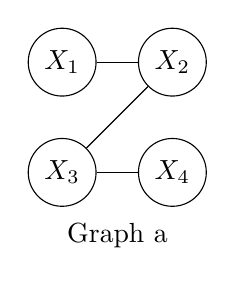
\begin{tikzpicture}
                            % Nodes
                            \foreach \i/\j/\k in {1/0/0, 2/1.4/0, 3/0/-1.4, 4/1.4/-1.4} {
                              \node[circle, draw, minimum size=8mm] (\i) at (\j,\k) {$X_{\i}$};
                            }
                            % Edges
                            \foreach \i [evaluate=\i as \j using int(\i+1)] in {1,2,3} {
                                \draw (\i) -- (\j);
                            }
                            % Label
                            \node[draw=none, fill=none] at (0.7,-2.2) {Graph a};
                        \end{tikzpicture}
                        \vskip10pt
                        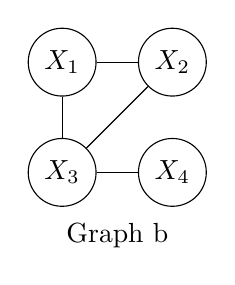
\begin{tikzpicture}
                            % Nodes
                            \foreach \i/\j/\k in {1/0/0, 2/1.4/0, 3/0/-1.4, 4/1.4/-1.4} {
                              \node[circle, draw, minimum size=8mm] (\i) at (\j,\k) {$X_{\i}$};
                            }
                            % Edges
                            \foreach \source/\target in {1/2, 2/3, 1/3, 3/4} {
                              \draw (\source) -- (\target);
                            }
                            \node[draw=none, fill=none] at (0.7,-2.2) {Graph b};
                        \end{tikzpicture}
                        \vskip10pt
                        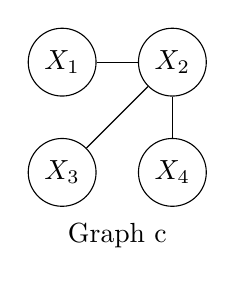
\begin{tikzpicture}
                            % Nodes
                            \foreach \i/\j/\k in {1/0/0, 2/1.4/0, 3/0/-1.4, 4/1.4/-1.4} {
                              \node[circle, draw, minimum size=8mm] (\i) at (\j,\k) {$X_{\i}$};
                            }
                            % Edges
                            \foreach \source/\target in {1/2, 2/3, 2/4} {
                              \draw (\source) -- (\target);
                            }
                            \node[draw=none, fill=none] at (0.7,-2.2) {Graph c};
                        \end{tikzpicture}
                    \end{center}
        \end{enumerate}
    \end{exercise}

    \newpage
    \textbf{\large \MBlue{Exercise 2}}
    \vskip10pt
    \noindent
	\begin{exercise}[Solution]
        \begin{enumerate}[(a)]
            \item We have the multivariate linear regression model given by
                    \begin{align*}
                        \Yv = \Xv B + E
                    \end{align*}
                    with $\Yv$ an $N\times m$ matrix, $\Xv$ an $N\times p$ matrix, $B$ a $p\times m$ matrix and $E$ a $N\times m$ matrix where each row $\epsilon_i^\top\overset{\text{i.i.d.}}{\sim}\mathcal{N}_m\left(0,\Sigma\right)$.\\
                    Now we have that
                    \begin{align*}
                        Y_i = B^\top X_i + \epsilon_i \sim \mathcal{N}_m\left(B^\top X_i, \Sigma\right)
                    \end{align*}
                    therefore our log-likelihood is given by
                    \begin{align*}
                        \ell\left(B,\Sigma\right) &= c + \frac{N}{2}\log\abs{\Sigma^{-1}} - \frac{1}{2}\tr{\sum_{i=1}^{N}\left(Y_i-B^\top X_i\right)^\top \Sigma^{-1}\left(Y_i-B^\top X_i\right)} = \\
                        &= c + \frac{N}{2}\log\abs{\Sigma^{-1}} - \frac{1}{2}\tr{\Sigma^{-1}\sum_{i=1}^{N}\left(Y_i-B^\top X_i\right)\left(Y_i-B^\top X_i\right)^\top} = \\
                        &= c + \frac{N}{2}\log\abs{\Sigma^{-1}} - \frac{1}{2}\tr{\Sigma^{-1} \left(\Yv-\Xv B\right)\left(\Yv-\Xv B\right)^\top}
                    \end{align*}
                    Now notice that our log-likelihood objective is strictly concave therefore setting the gradients with respect to our parameters yields the unique maximizer. Moreover, setting the gradient with respect to $\Sigma$ to 0 is equivalent to setting the gradient with respect to $\Sigma^{-1}$ to 0.\\
                    Therefore taking the gradients with respect to $B$ and $\Sigma^{-1}$ yields
                    \begin{align*}
                        \nabla_B \ell\left(B,\Sigma\right) &= -\frac{1}{2}\nabla_B \tr{\Sigma^{-1} \left(\Yv-\Xv B\right)\left(\Yv-\Xv B\right)^\top} = \\
                        &= -\frac{1}{2}\left[\nabla_B\left(\Yv-\Xv B\right)\right] \left(\Yv-\Xv B\right)\left(\Sigma^{-1}+\Sigma^{-1}\right) = \\
                        &= \Xv^\top\left(\Yv-\Xv B\right)\Sigma^{-1} \overset{!}{=} 0 \implies \\
                        \hat{B} &= \left(\Xv^\top\Xv\right)^{-1}\Xv^\top\Yv\\
                        \nabla_{\Sigma^{-1}} \ell\left(B,\Sigma\right) &= \frac{N}{2} \Sigma ^\top -\frac{1}{2} \left(\Yv-\Xv B\right)^\top\left(\Yv-\Xv B\right) = \\
                        &=\frac{N}{2} \Sigma -\frac{1}{2} \left(\Yv-\Xv B\right)^\top\left(\Yv-\Xv B\right) = 0\implies\\
                        \hat{\Sigma} &= \frac{1}{N}\left(\Yv-\Xv \hat{B}\right)^\top\left(\Yv-\Xv \hat{B}\right) = \\
                        &= \frac{1}{N}\left(\Yv-\Xv \left(\Xv^\top\Xv\right)^{-1}\Xv^\top\Yv\right)^\top\left(\Yv-\Xv \left(\Xv^\top\Xv\right)^{-1}\Xv^\top\Yv\right) = \\
                        &= \frac{1}{N}\Yv^\top \left(\Id_N - \Xv \left(\Xv^\top\Xv\right)^{-1}\Xv^\top\right)^\top\left(\Id_N - \Xv \left(\Xv^\top\Xv\right)^{-1}\Xv^\top\right)\Yv = \\
                        &= \frac{1}{N}\Yv^\top \left(\Id_N - \Xv \left(\Xv^\top\Xv\right)^{-1}\Xv^\top\right)\Yv
                    \end{align*}
                    Therefore
                    \begin{align*}
                        \hat{B} &= \left(\Xv^\top\Xv\right)^{-1}\Xv^\top\Yv\\
                        \hat{\Sigma} &= \frac{1}{N}\Yv^\top \left(\Id_N - \Xv \left(\Xv^\top\Xv\right)^{-1}\Xv^\top\right)\Yv
                    \end{align*}
            \item Now we define the $\text{RSS}$ as 
                    \begin{align*}
                        \text{RSS}(B) = \sum_{i=1}^{N} \left(Y_i^\top - X_i^\top B\right)\left(Y_i^\top - X_i^\top B\right)^\top
                    \end{align*}
                    Then taking the gradient with respect to $B$ we have
                    \begin{align*}
                        \nabla_B\text{RSS}(B) &= \sum_{i=1}^{N}-2\left[\nabla_B\left(Y_i^\top - X_i^\top B\right)\right]\left(Y_i^\top - X_i^\top B\right) = \\
                        &= \sum_{i=1}^{N}-2 X_i \left(Y_i^\top - X_i^\top B\right) = \\
                        &= -2\sum_{i=1}^{N}X_i Y_i^\top + 2 \left(\sum_{i=1}^{N} X_i X_i^\top\right) B = \\
                        &= -2 \Xv^\top\Yv + 2 \Xv^\top\Xv B = 0 \implies\\
                        \hat{B} &= \left(\Xv^\top\Xv\right)^{-1}\Xv^\top\Yv
                    \end{align*}
                    thus yielding the same estimator as the MLE from part (a).
        \end{enumerate}
    \end{exercise}

    \newpage
    \textbf{\large \MBlue{Exercise 3}}
    \vskip10pt
    \noindent
	\begin{exercise}[Solution]
        Code is also available at \url{https://github.com/paoloborello/601W24/tree/main/HW_1/code}
    \end{exercise}

    \newpage
    \textbf{\large \MBlue{Exercise 4}}
    \vskip10pt
    \noindent
	\begin{exercise}[Solution]
        \begin{enumerate}[(a)]
            \item We know from lecture that the MLE for $\left(\mu,\Sigma\right)$ when $X_i\overset{\text{i.i.d.}}{\sim}\mathcal{N}_p\left(\mu,\Sigma\right)$ is given by $\left(\bar{X}_N, S_N\right)$, where $\bar{X}_N$ is the sample mean vector and $S_N$ is the uncorrected sample covariance matrix.\\
                    Therefore to get the LRT we still need to find the MLE under the null hypothesis
                    \begin{align*}
                        H_0: \mu=0
                    \end{align*}
                    therefore we want to solve
                    \begin{align*}
                        \argmax_{\Sigma} \ell(0,\Sigma) &= \argmax_{\Sigma}-\frac{N}{2}\log\abs{\Sigma}-\frac{1}{2}\sum_{i=1}^{N}X_i^\top\Sigma^{-1}X_i = \\
                        &= \argmax_{\Sigma}-N\tr{\log\abs{\Sigma}}-\sum_{i=1}^{N}\tr{X_i^\top\Sigma^{-1}X_i} = \\
                        &= \argmax_{\Sigma}N\tr{\log\abs{\Sigma^{-1}}}-\sum_{i=1}^{N}\tr{\Sigma^{-1}X_i X_i^\top}
                    \end{align*}
                    then taking the gradient with respect to $\Sigma^{-1}$ (this suffices to find the maximum by the same argument as in exercise 2) yields 
                    \begin{align*}
                        \nabla_{\Sigma^{-1}}\ell(\Sigma) = N\Sigma - \sum_{i=1}^{N} \left(X_i X_i^\top\right)^\top = 0 \implies \hat{\Sigma}_0 = \frac{1}{N}\sum_{i=1}^{N} X_i^\top X_i
                    \end{align*}
                    Thus the LRT takes the following form 
                    \begin{align*}
                        T_{\text{LRT}} &= -2\left[\ell\left(0,\hat{\Sigma}_0\right)-\ell\left(\bar{X}_n,S_N\right)\right] = \\
                        &= N\log\abs{\hat{\Sigma}_0}+\sum_{i=1}^{N}X_i^\top\hat{\Sigma}_0^{-1}X_i - N\log\abs{S_N}+\sum_{i=1}^{N}\left(X_i-\bar{X}_N\right)^\top S_N^{-1}\left(X_i-\bar{X}_N\right) = \\
                        &= N\log\frac{\abs{\hat{\Sigma}_0}}{\abs{S_N}} + \sum_{i=1}^{N} X_i^\top\hat{\Sigma}_0^{-1}X_i - \left(X_i-\bar{X}_N\right)^\top S_N^{-1}\left(X_i-\bar{X}_N\right)
                    \end{align*}
                    Now notice that
                    \begin{align*}
                        S_N &= \frac{1}{N}\sum_{i=1}^{N}\left(X_i-\bar{X}_N\right)\left(X_i-\bar{X}_N\right)^\top = \\
                        &= \frac{1}{N}\sum_{i=1}^{N}X_i X_i^\top - \bar{X}_N X_i^\top - X_i\bar{X}_N^\top + \bar{X}_N\bar{X}_N^\top = \\
                        &= \left(\frac{1}{N}\sum_{i=1}^{N}X_i X_i^\top\right) - \bar{X}_N \bar{X}_N^\top - \bar{X}_N \bar{X}_N^\top + \bar{X}_N\bar{X}_N^\top = \\
                        &= \hat{\Sigma}_0 - \bar{X}_N \bar{X}_N^\top
                    \end{align*}
                    Then applying the \href{https://en.wikipedia.org/wiki/Matrix_determinant_lemma}{matrix determinant lemma} we have that
                    \begin{align*}
                        \abs{\hat{\Sigma}_0} = \abs{S_N + \bar{X}_N \bar{X}_N^\top} = \abs{S_N}\left(1+\bar{X}_N^\top S_N^{-1}\bar{X}_N\right)
                    \end{align*}
                    therefore
                    \begin{align*}
                        \frac{\abs{\hat{\Sigma}_0}}{\abs{S_N}} = 1+\bar{X}_N^\top S_N^{-1}\bar{X}_N
                    \end{align*}
                    Now moving to the sample covariance $\tilde{S}_N$ we have that
                    \begin{align*}
                        \tilde{S}_N = \frac{N}{N-1}S_N
                    \end{align*}
                    therefore
                    \begin{align*}
                        \frac{\abs{\hat{\Sigma}_0}}{\abs{S_N}} = 1+N\bar{X}_N^\top \tilde{S}_N^{-1}\bar{X}_N\frac{1}{N-1}= 1+\frac{T^2}{N-1}
                    \end{align*}
                    then by \href{https://en.wikipedia.org/wiki/Sherman%E2%80%93Morrison_formula}{Sherman-Morisson formula} we have that
                    \begin{align*}
                        \hat{\Sigma}_0^{-1} &= \left(S_N + \bar{X}_N \bar{X}_N^\top\right)^{-1} = S_N^{-1} - \frac{S_N^{-1}\bar{X}_N \bar{X}_N^\top S_N^{-1}}{1+ \bar{X}_N^\top S_N^{-1}\bar{X}_N}
                    \end{align*}
                    therefore
                    \begin{gather*}
                        \sum_{i=1}^{N} X_i^\top\hat{\Sigma}_0^{-1}X_i - \left(X_i-\bar{X}_N\right)^\top S_N^{-1}\left(X_i-\bar{X}_N\right) =\\
                        = \sum_{i=1}^{N} X_i^\top S_N^{-1}X_i - X_i^\top \frac{S_N^{-1}\bar{X}_N \bar{X}_N^\top S_N^{-1}}{1+ \bar{X}_N^\top S_N^{-1}\bar{X}_N} X_i - \left(X_i-\bar{X}_N\right)^\top S_N^{-1}\left(X_i-\bar{X}_N\right) = \\
                        = \left(-\sum_{i=1}^{N} X_i^\top \frac{S_N^{-1}\bar{X}_N \bar{X}_N^\top S_N^{-1}}{1+ \bar{X}_N^\top S_N^{-1}\bar{X}_N} X_i\right) + N  \bar{X}_N^\top S_N^{-1}\bar{X}_N
                    \end{gather*}
                    Now
                    \begin{align*}
                        -\sum_{i=1}^{N} X_i^\top \frac{S_N^{-1}\bar{X}_N \bar{X}_N^\top S_N^{-1}}{1+ \bar{X}_N^\top S_N^{-1}\bar{X}_N} X_i &= - \tr{\sum_{i=1}^{N}X_i^\top \frac{S_N^{-1}\bar{X}_N \bar{X}_N^\top S_N^{-1}}{1+ \bar{X}_N^\top S_N^{-1}\bar{X}_N} X_i} =\\
                        &= -\frac{1}{1+ \bar{X}_N^\top S_N^{-1}\bar{X}_N}\tr{S_N^{-1}\bar{X}_N \bar{X}_N^\top S_N^{-1} \sum_{i=1}^{N}X_i X_i^\top} =\\
                        &= -\frac{1}{1+ \bar{X}_N^\top S_N^{-1}\bar{X}_N}\tr{N S_N^{-1}\bar{X}_N \bar{X}_N^\top S_N^{-1} \hat{\Sigma}_0} = \\
                        &= -\frac{N}{1+ \bar{X}_N^\top S_N^{-1}\bar{X}_N}\tr{S_N^{-1}\bar{X}_N \bar{X}_N^\top S_N^{-1} \left(S_N + \bar{X}_N \bar{X}_N^\top\right)} = \\
                        &= -\frac{N}{1+ \bar{X}_N^\top S_N^{-1}\bar{X}_N}\tr{S_N^{-1}\bar{X}_N \bar{X}_N^\top + S_N^{-1}\bar{X}_N \bar{X}_N^\top S_N^{-1}\bar{X}_N \bar{X}_N^\top} = \\
                        &= -\frac{N}{1+ \bar{X}_N^\top S_N^{-1}\bar{X}_N}\tr{\bar{X}_N^\top S_N^{-1}\bar{X}_N + \bar{X}_N^\top S_N^{-1}\bar{X}_N\bar{X}_N^\top S_N^{-1}\bar{X}_N} = \\
                        &= -\frac{N}{1+ \bar{X}_N^\top S_N^{-1}\bar{X}_N}\tr{\left(1+\bar{X}_N^\top S_N^{-1}\bar{X}_N\right) \bar{X}_N^\top S_N^{-1}\bar{X}_N} = \\
                        &= -N\bar{X}_N^\top S_N^{-1}\bar{X}_N
                    \end{align*}
                    thus
                    \begin{align*}
                        \sum_{i=1}^{N} X_i^\top\hat{\Sigma}_0^{-1}X_i - \left(X_i-\bar{X}_N\right)^\top S_N^{-1}\left(X_i-\bar{X}_N\right) = - N \bar{X}_N^\top S_N^{-1}\bar{X}_N + N \bar{X}_N^\top S_N^{-1}\bar{X}_N = 0
                    \end{align*}
                    therefore the LRT is 
                    \begin{align*}
                        T_{\text{LRT}} &= N\log\left(1+\frac{T^2}{N-1}\right) = -N\log\frac{1}{1+\frac{T^2}{N-1}}
                    \end{align*}
                    then the likelihood Ratio itself is given by
                    \begin{align*}
                        \frac{\mathcal{L}\left(0,\hat{\Sigma}_0\right)}{\mathcal{L}\left(\bar{X}_N,S_N\right)} = \exp\left\{-\frac{T_{\text{LRT}}}{2}\right\} = \exp\left\{\frac{N}{2}\log\frac{1}{1+\frac{T^2}{N-1}}\right\} = \left(\frac{1}{1+\frac{T^2}{N-1}}\right)^{N/2}
                    \end{align*}
            \item Since $S_N$ is p.s.d. by construction
                    \begin{align*}
                        T^2 = N\bar{X}_N^\top S_N^{-1}\bar{X}_N = N\bar{X}_N^\top S_N^{-1/2} S_N^{-1/2}\bar{X}_N = \norm{\sqrt{N}S_N^{-1/2}\bar{X}_N}_2^2
                    \end{align*}
                    Under $H_0:\mu=0$, we have
                    \begin{align*}
                        \sqrt{N}\bar{X}_N&\overset{\text{d}}{\longrightarrow}\mathcal{N}_p(0,\Sigma)\\
                        S_N&\overset{\mathbb{P}}{\longrightarrow}\Sigma \implies S_N^{-1/2}\overset{\mathbb{P}}{\longrightarrow}\Sigma^{-1/2}
                    \end{align*}
                    then by Slutsky
                    \begin{align*}
                        \sqrt{N}S_N^{-1/2}\bar{X}_N\overset{\text{d}}{\longrightarrow}\mathcal{N}_p\left(0,\Id_p\right)\implies \norm{\sqrt{N}S_N^{-1/2}\bar{X}_N}_2^2\overset{\text{d}}{\longrightarrow}\chi^2_p
                    \end{align*}
            \item For each significance level, I plot the empirical estimate of type I error
                    \begin{center}
                        \includegraphics[width=.7\linewidth]{ex4_3.png}
                    \end{center}
                    I ran 1000 replications and we can see that we are quite able to control for type I error at all significance levels.
            \item For each significance level, I plot the empirical estimate of type I error
                    \begin{center}
                        \includegraphics[width=.7\linewidth]{ex4_10.png}
                        \includegraphics[width=.7\linewidth]{ex4_40.png}
                        \includegraphics[width=.7\linewidth]{ex4_80.png}
                    \end{center}
                    Now we can see that as dimesionality increases we are not able to control for type I error anymore.
            \item Let $\left\{a_j\right\}_{j\in\left[p\right]}$ and $\left\{b_k\right\}_{k\in\left[N-p\right]}$ be two sequences of independent $\chi_1^2$ rvs. Then
                    \begin{align*}
                        \mean{a_j} &= \mean{b_k} = 1\\
                        \var{a_j} &= \var{b_k} = 2
                    \end{align*}
                    therefore
                    \begin{align*}
                        \bar{a}&\coloneq\frac{1}{p}\sum_{j=1}^{p}a_j\sim\frac{\chi_p^2}{p}\\
                        \bar{b}&\coloneq\frac{1}{N-p}\sum_{k=1}^{N-p}b_k\sim\frac{\chi_{N-p}^2}{N-p}
                    \end{align*}
                    By the Central Limit Theorem we have 
                    \begin{align*}
                        \sqrt{p}(\bar{a}-1)&\overset{d}{\longrightarrow}\mathcal{N}(0,2), p\rightarrow\infty\\
                        \sqrt{N-p}(\bar{b}-1)&\overset{d}{\longrightarrow}\mathcal{N}(0,2), N\rightarrow\infty, p\rightarrow\infty, \frac{p}{N}\longrightarrow\gamma\in(0,1)
                    \end{align*}
                    which implies
                    \begin{align*}
                        \sqrt{N}(\bar{a}-1)&\overset{d}{\longrightarrow}\mathcal{N}\left(0,\frac{2}{\gamma}\right)\\
                        \sqrt{N}(\bar{b}-1)&\overset{d}{\longrightarrow}\mathcal{N}\left(0,\frac{2}{1-\gamma}\right)
                    \end{align*}
                    and by independence we have
                    \begin{align*}
                        \sqrt{N}
                        \begin{pmatrix}
                            \begin{pmatrix}
                                \bar{a}\\
                                \bar{b}
                            \end{pmatrix}-
                            \begin{pmatrix}
                                1\\
                                1
                            \end{pmatrix}
                        \end{pmatrix}
                        \overset{d}{\longrightarrow}\mathcal{N}_2
                        \begin{pmatrix}
                            \begin{pmatrix}
                                0\\
                                0
                            \end{pmatrix},
                            \begin{pmatrix}
                                \frac{2}{\gamma} & 0\\
                                0 & \frac{2}{1-\gamma}
                            \end{pmatrix}
                        \end{pmatrix}
                    \end{align*}
                    Then let $g(x,y) = x/y$ 
                    \begin{align*}
                        \nabla g(x,y) &=
                        \begin{pmatrix}
                            \frac{1}{y}\\
                            -\frac{x}{y^2}
                        \end{pmatrix}\\
                        \nabla g(1,1) &=
                        \begin{pmatrix}
                            1\\
                            -1
                        \end{pmatrix}\\
                        \nabla g(1,1)^\top 
                        \begin{pmatrix}
                            \frac{2}{\gamma} & 0\\
                            0 & \frac{2}{1-\gamma}
                        \end{pmatrix}
                        \nabla g(1,1) &= \frac{2}{\gamma}+\frac{2}{1-\gamma}=\\
                        &= \frac{2}{\gamma(1-\gamma)}
                    \end{align*}
                    and using the delta method
                    \begin{align*}
                        \sqrt{N}\left(\frac{\bar{a}}{\bar{b}}-1\right)\overset{d}{\longrightarrow}\mathcal{N}\left(0,\frac{2}{\gamma(1-\gamma)}\right)
                    \end{align*}
                    Now since 
                    \begin{align*}
                        \frac{\bar{a}}{\bar{b}}\sim\frac{\chi_p^2}{\chi_{N-p}^2} \overset{d}{=} F_{p,N-p} \sim \frac{N-p}{p(N-1)}T^2
                    \end{align*}
                    then
                    \begin{align*}
                        \sqrt{N}\left(\frac{N-p}{p(N-1)}T^2-1\right)\overset{d}{\longrightarrow}\mathcal{N}\left(0,\frac{2}{\gamma(1-\gamma)}\right)
                    \end{align*}
            \item In the case that $p>N$, then our design matrix will not be full rank and hence $S_N$ will not be invertible, thus we cannot compute $T^2$.
        \end{enumerate}
    \end{exercise}

\end{document}